%%
%  ******************************************************************************
%  * #file    Szablon_raportu_EN_Latex.tex
%  * #author  Adrian Wójcik   adrian.wojcik(at)put.poznan.pl
%  *          
%  * #commit  Patryk Kościk   koscikpatryk(at)gmail.com
%  *          Modified the template for Projekt przejsciowy purposes          
%  *          
%  * #version 1.0
%  * #date    09-Mar-2022
%  * #brief   PROJPRZEJ
%  *
%  ******************************************************************************
%%  
\documentclass[11pt, a4paper]{article}

\usepackage{Szablon_raportu_EN_Latex}

% Wypełnijcie te dyrektywy zgodnie z waszym tematem
% \lab      -> NAZWA CZUJNIKA, np.: 'DHT22'
% \comment  -> Króciutki opis co to, np.: 'Cyfrowy budżetowy czujnik temperatury'
%
\lab{Moduł KY-019}
\comment{Przekaźnik sterowany napięciem 5V}

% Absolutny zakaz dotykania tego tutaj bo jak dotkiecie to coś jebnie
\university{Politechnika Poznańska}
\faculty{Wydział Automatyki, Robotyki i Elektrotechniki}
\institute{Instytut Robotyki i Inteligencji Maszynowej}
\department{Zakład Sterowania i Elektroniki Przemysłowej}
\addbibresource{Szablon_raportu_EN_Latex.bib}
\nocite{*}


%%
%
% Początek dokumentu
%
%%
\begin{document}

%% Strona tytułowa %%
\mainpage{przekaznik}
\newpage

\section*{Opis elementu} \addcontentsline{toc}{section}{Wstęp}
Moduł przekaźnika KY-019 składa się z trzech pinów męskich, z czego dwa służą do zasilania cewki, a  trzeci to styk sterujący tzw. signal.
Wyposażenie dopełniają dioda LED sygnalizująca podłączenie zasilania i dioda prostownicza zapobiegająca przepięciom.
Parametry przekaźnika to: 10A 250VAC 10A 30V DC, 10A 125VAC 10A 28VDC


\vspace{0.5cm}
\begin{figure}[h]
\centering
\begin{subfigure}{.5\textwidth}
  \centering
  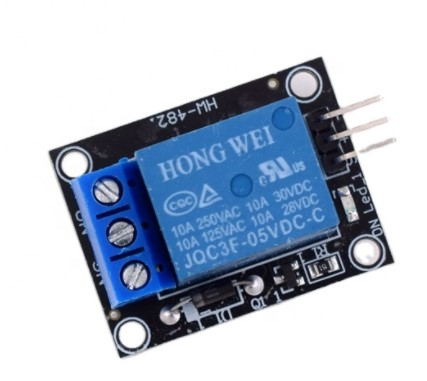
\includegraphics[width=.4\linewidth]{fig/obrazki/zdj_modułu/przod.jpg}
  \caption{frontalny pogląd na przekaźnik}
  \label{fig:sub1}
\end{subfigure}%
\begin{subfigure}{.5\textwidth}
  \centering
  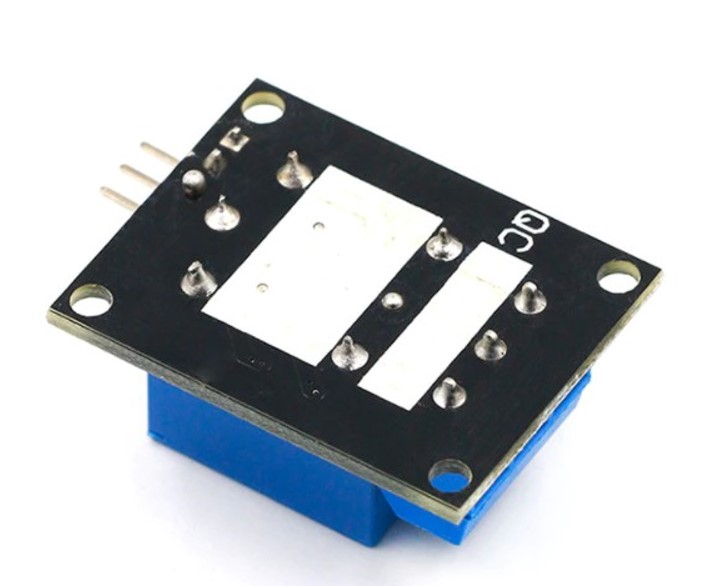
\includegraphics[width=.4\linewidth]{fig/obrazki/zdj_modułu/tył_.jpg}
  \caption{Podgląd na tylnią część}
  \label{fig:sub2}
\end{subfigure}
\caption{podgląd na KY-019 z obu stron}
\label{fig:test}
\end{figure}
\vspace{0.5cm}

%\subsection{Zasada działania}
Moduł zasilamy podając napięcie 5V na pin oznaczony symbolem "$+$", masę GND do pinu opisanego "$-$" i pin \textbf{s} tzw. signal. Przy podaniu 5V na pin \textbf{s} jesteśmy w stanie sterować przekaźnikiem, by poprzez wytworzone pole magnetyczne przez cewkę przekazać sygnał na wyjście przekaźnika. Urządzenie ma trzy wyjścia, środkowy tzw. "wspólny", wyjście normalnie otwarte (NO) i wyjście normalnie zamknięte (NC). Wyjścia wykorzystujemy do zasilania kolejnego układu (na przykład zasilanego prądem przemiennym o wysokiej częstotliwości )

\vspace{0.5cm}
\begin{figure}[h]
\centering
\begin{subfigure}{.5\textwidth}
  \centering
  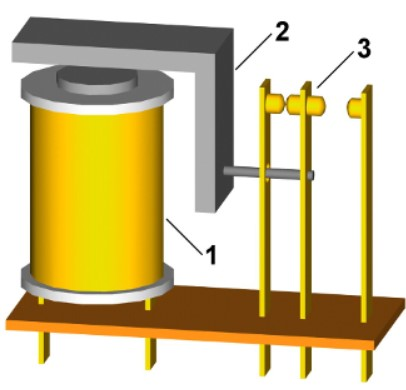
\includegraphics[width=.4\linewidth]{fig/obrazki/zasada_dzialania/1faza.jpg}
  \caption{Przekaźnik w stanie zamknięcia obwodu NO}
  \label{fig:sub1}
\end{subfigure}%
\begin{subfigure}{.5\textwidth}
  \centering
  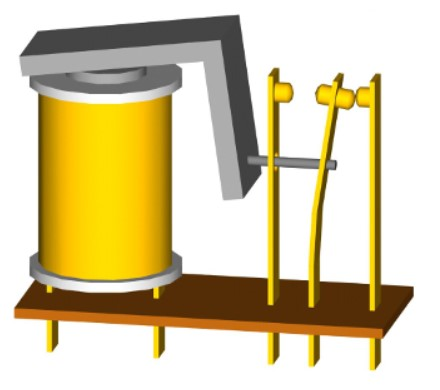
\includegraphics[width=.4\linewidth]{fig/obrazki/zasada_dzialania/2faza.jpg}
  \caption{Przekaźnik w stanie zamknięcia obwod NC}
  \label{fig:sub2}
\end{subfigure}
\caption{Dwa przyciski}
\label{fig:test}
\end{figure}
\vspace{0.5cm}

%\subsection{Zastosowania}
Przekaźniki są bardzo popularnym i często wykorzystywanym elementem przede wszystkim przemyśle (np. automatyce).
Mamy jednak z nimi do czynienia w życiu codziennym, odpowiadają bowiem one za prawidłowe sterowanie sygnalizacją świetlna, ruchomymi schodami, wiatrakami, czy też windami. Są one również bardzo ważnym elementem w nowych systemach, na przykład smart dom.


\newpage

%\section{Implementacja czujnika}


% \vspace{0.5cm}

% \vspace{0.5cm}
% \begin{figure}[h!]
%     \centering
%     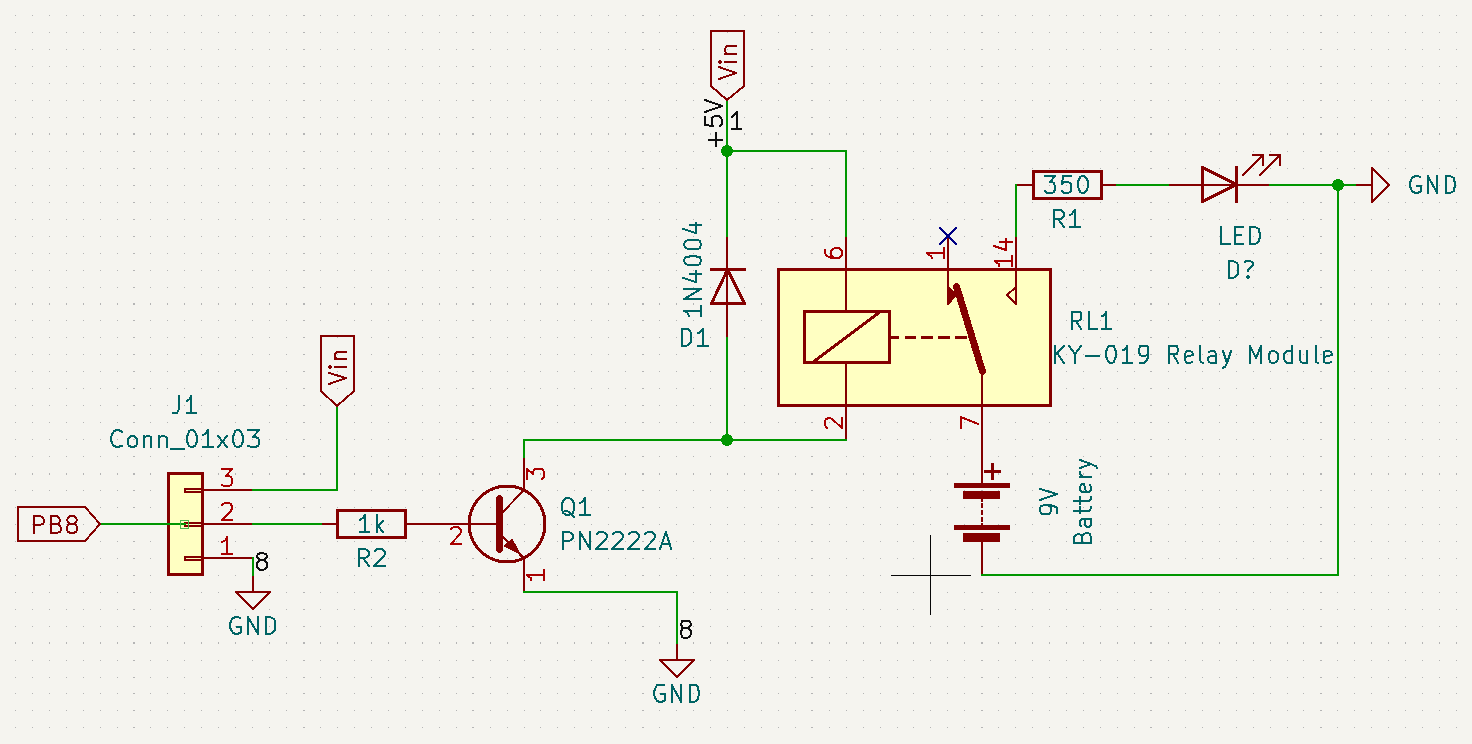
\includegraphics[scale=0.53]{fig/obrazki/polaczenie_modulu/Schematki.png}
%     \caption{Połaczenie elektryczne}
%     \label{fig:my_label}
% \end{figure}
% \vspace{0.5cm}


\newpage

%\section{Prezentacja działania układu}
\section{Użycie czujnika}

% \vspace{0.5cm}
% \begin{figure}[h!]
%     \centering
%     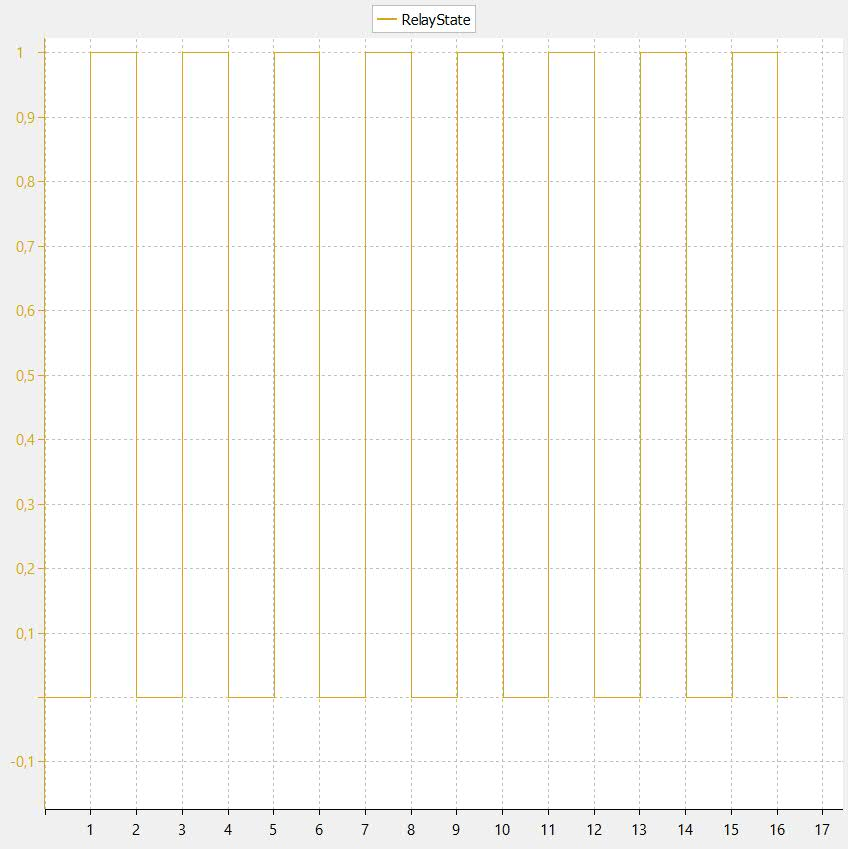
\includegraphics[width=0.6\textwidth]{fig/obrazki/działanie_ukladu/SWV.jpeg}
%     \caption{Przykładowy zrzut ekranu z SWV}
%     \label{fig:my_label}
% \end{figure}
% \vspace{0.5cm}

% W określonych chwilach czasowych (tutaj przykładowo 1 sekunda) dzięki pinowi sterującemu, przekazujemy (lub też nie) sygnał na wyjście przekaźnika, co obserwujemy zmieniającym się stanem zmiennej \textbf{RelayState}

\vspace{0.5cm}
\begin{figure}[h!]
    \centering
    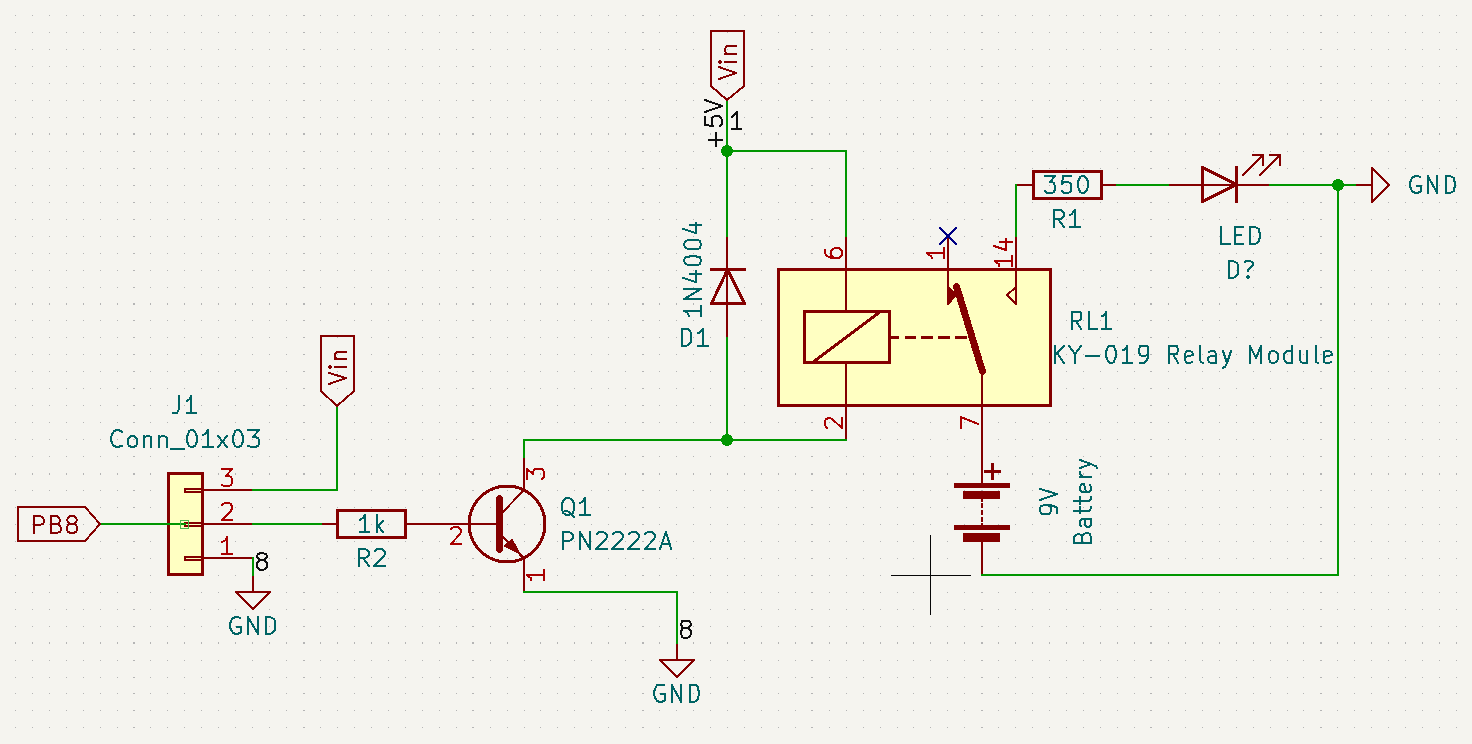
\includegraphics[scale=0.53]{fig/obrazki/polaczenie_modulu/Schematki.png}
    \caption{Połaczenie elektryczne}
    \label{fig:my_label}
\end{figure}
\vspace{0.5cm}

Na powyższym rysunku obserwujemy ogólny schemat elektryczny modułu KY-019. Zwracamy uwagę, że mamy zależność pomiędzy napięciem zasilania a pinem sterującym PB8. Dzięki tej zależności w odpowiednich chwilach możemy sterować naszym przekaźnikiem.

\newpage

\vspace{0.5cm}
\begin{figure}[h!]
    \centering
    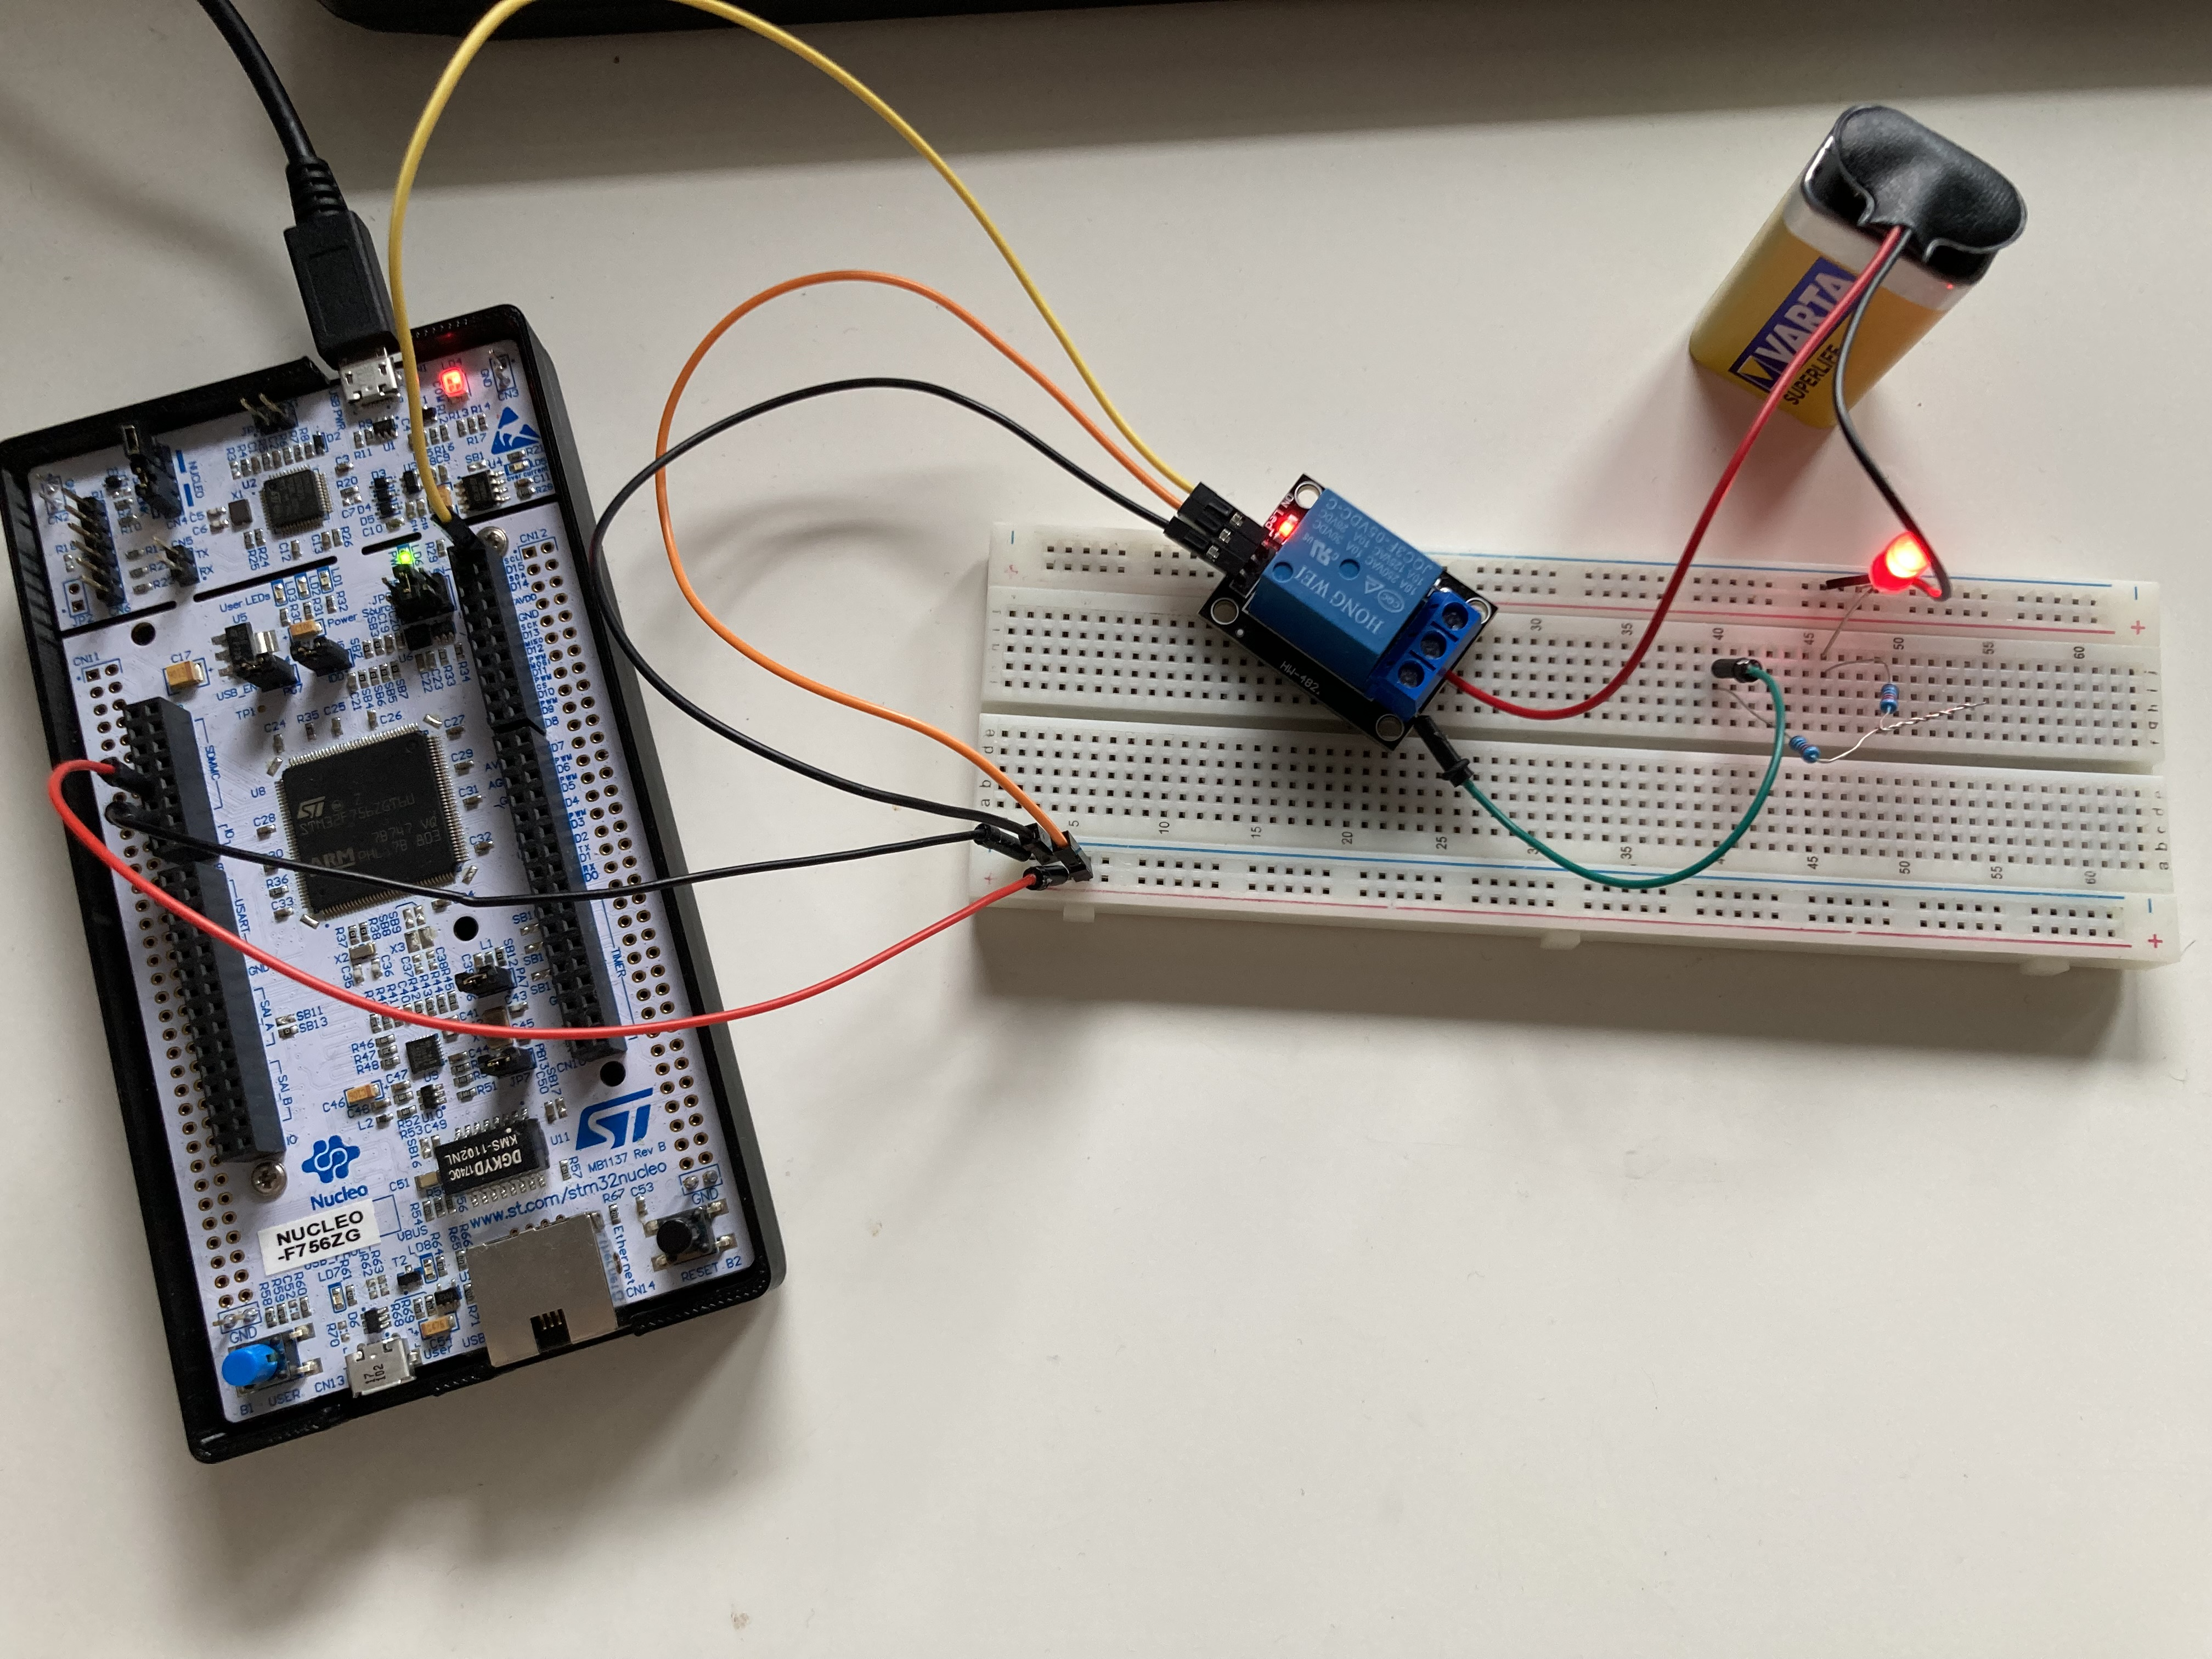
\includegraphics[scale=0.1]{fig/obrazki/działanie_ukladu/CALOSC2.jpg}
    \caption{Rzeczywista realizacja układu}
    \label{fig:my_label}
\end{figure}
\vspace{0.5cm}

Na załączonej fotografii obserwujemy układ z przekaźnikiem oraz dodatkowym obwodem zawierającym zasilanie z baterii 9V, rezystor 350$\Omega$ oraz diodę LED. Ten sposób realizacji ma pokazać zastosowanie przekaźnika, który sterując małym napięcem potrafi załączyć inny układ o przypuszczalnie większym napięciu.

\newpage

\vspace{0.5cm}
\begin{figure}[h!]
    \centering
    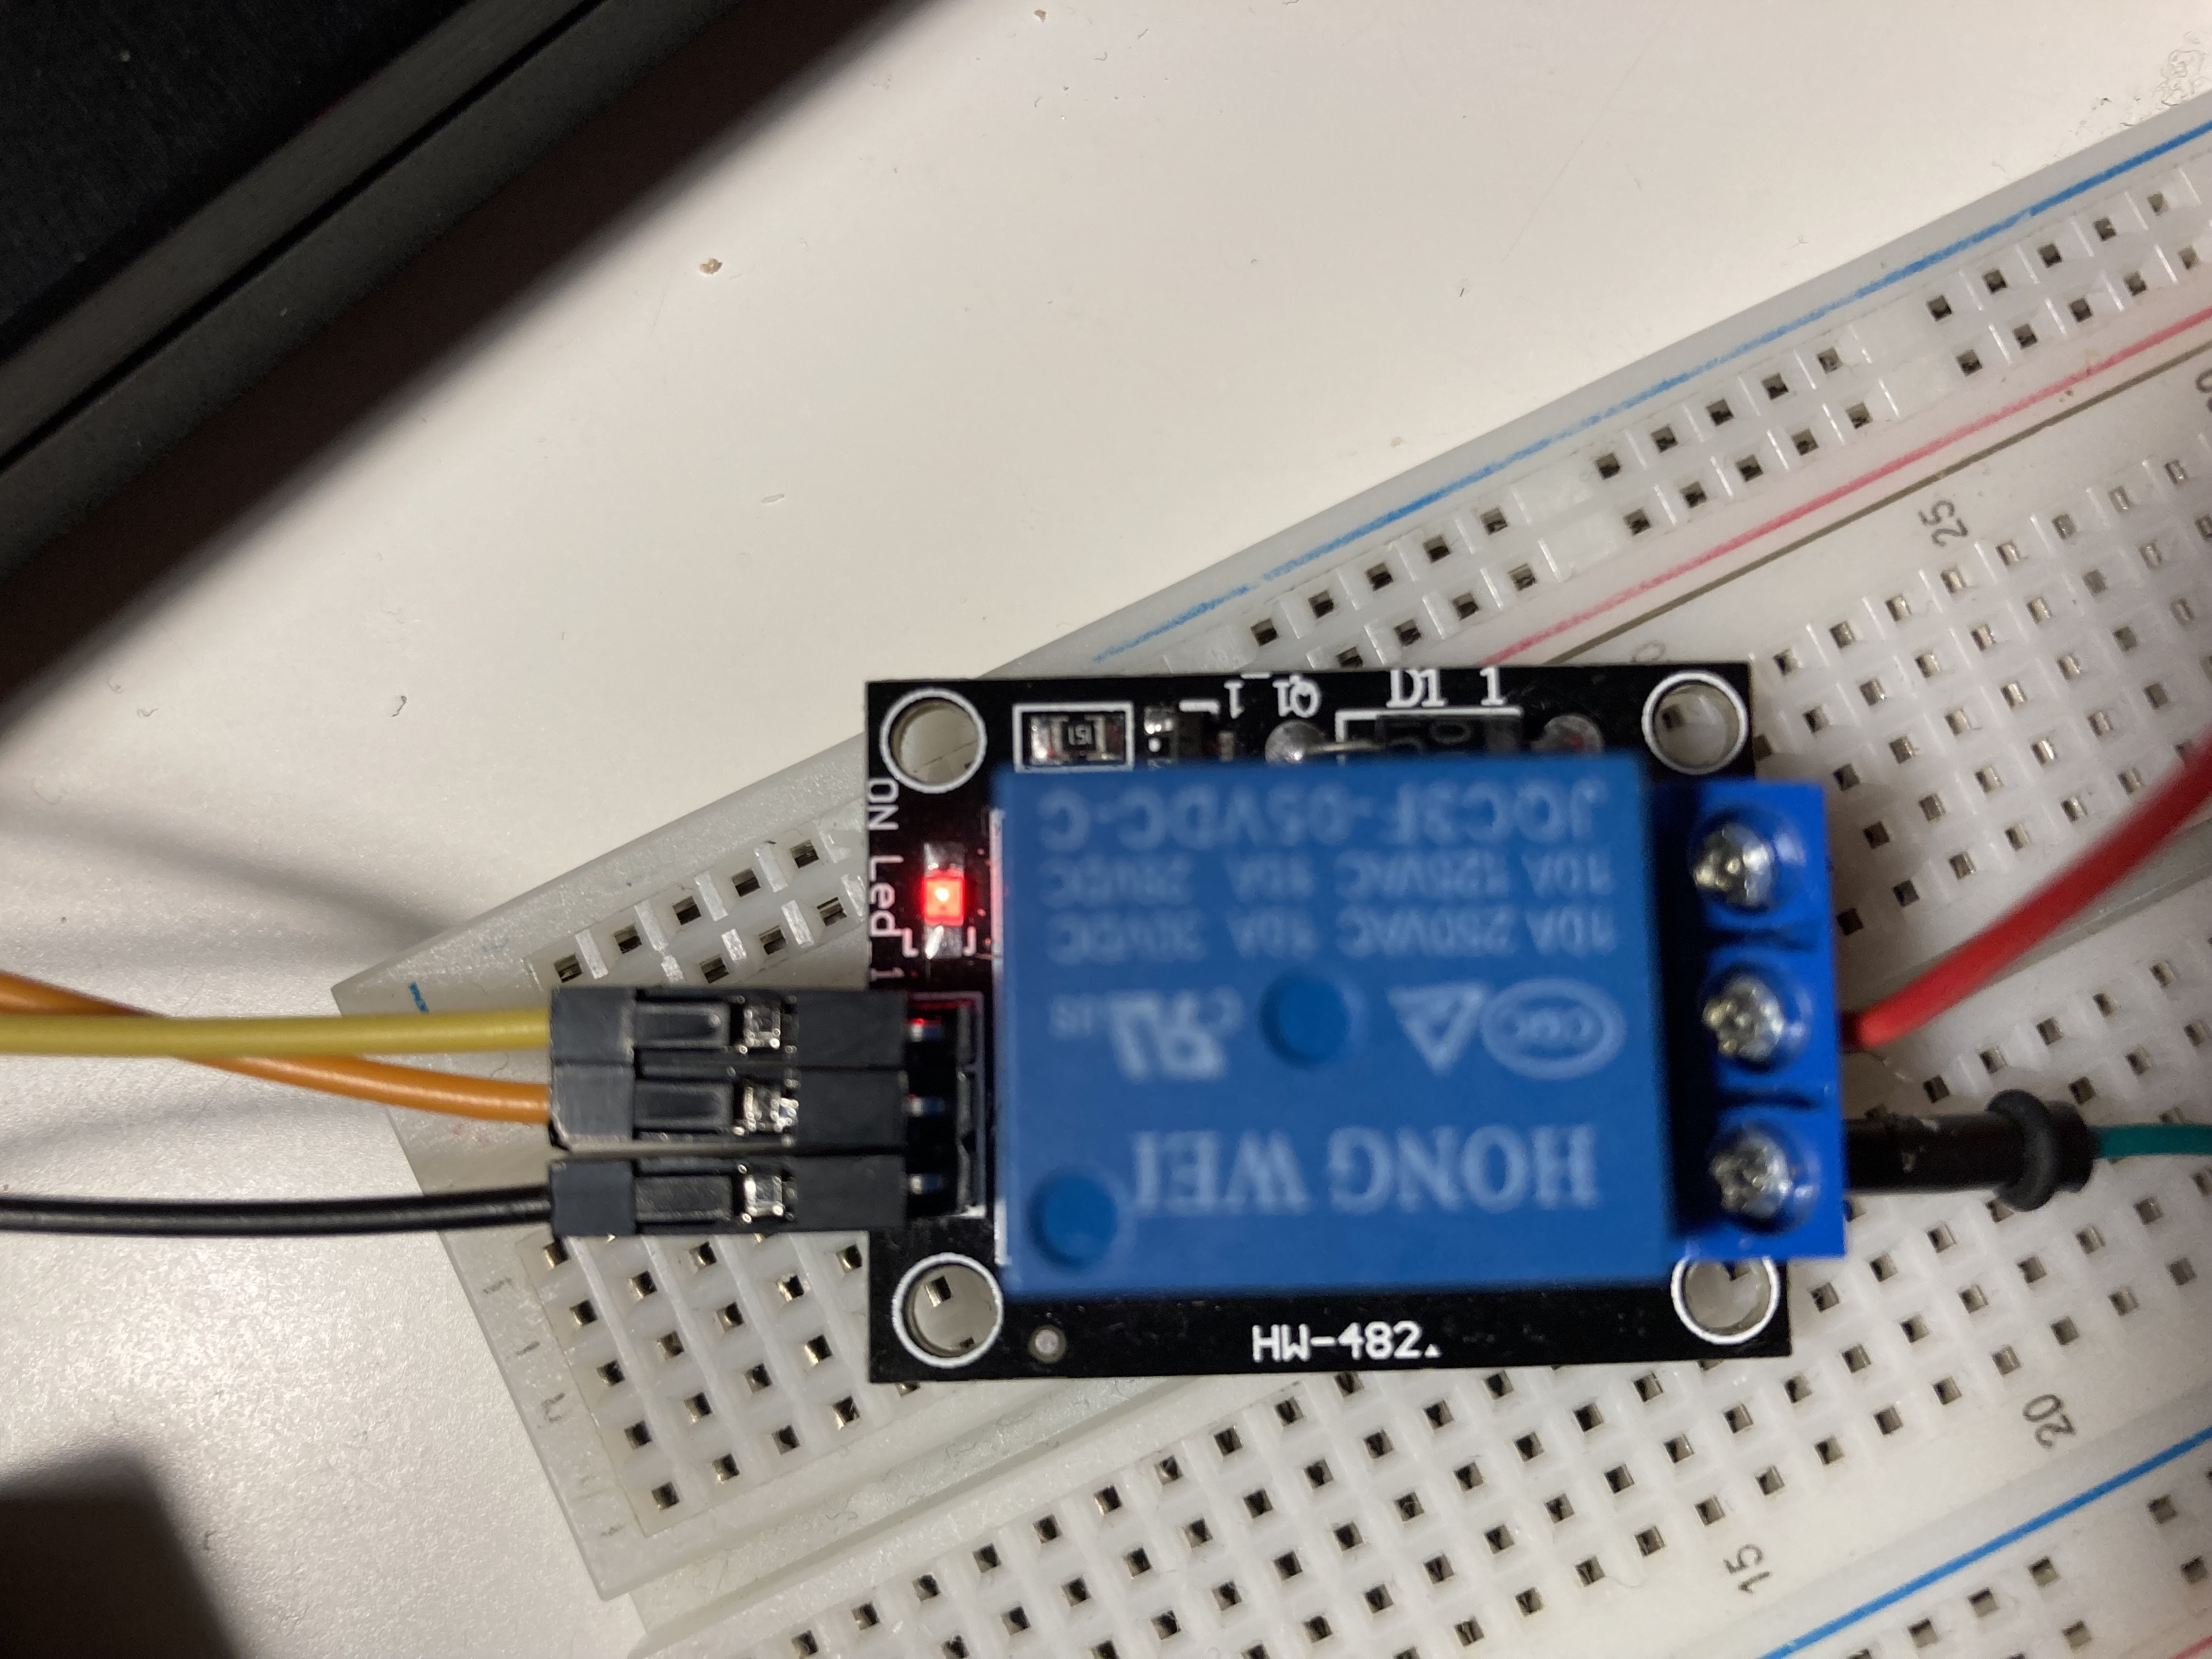
\includegraphics[scale=0.08]{fig/obrazki/działanie_ukladu/bliskoon.jpg}
    \caption{dioda LED sygnalizująca podłączenie zasilania}
    \label{fig:my_label}
\end{figure}
\vspace{0.5cm}


\vspace{0.5cm}
\begin{figure}[h!]
    \centering
    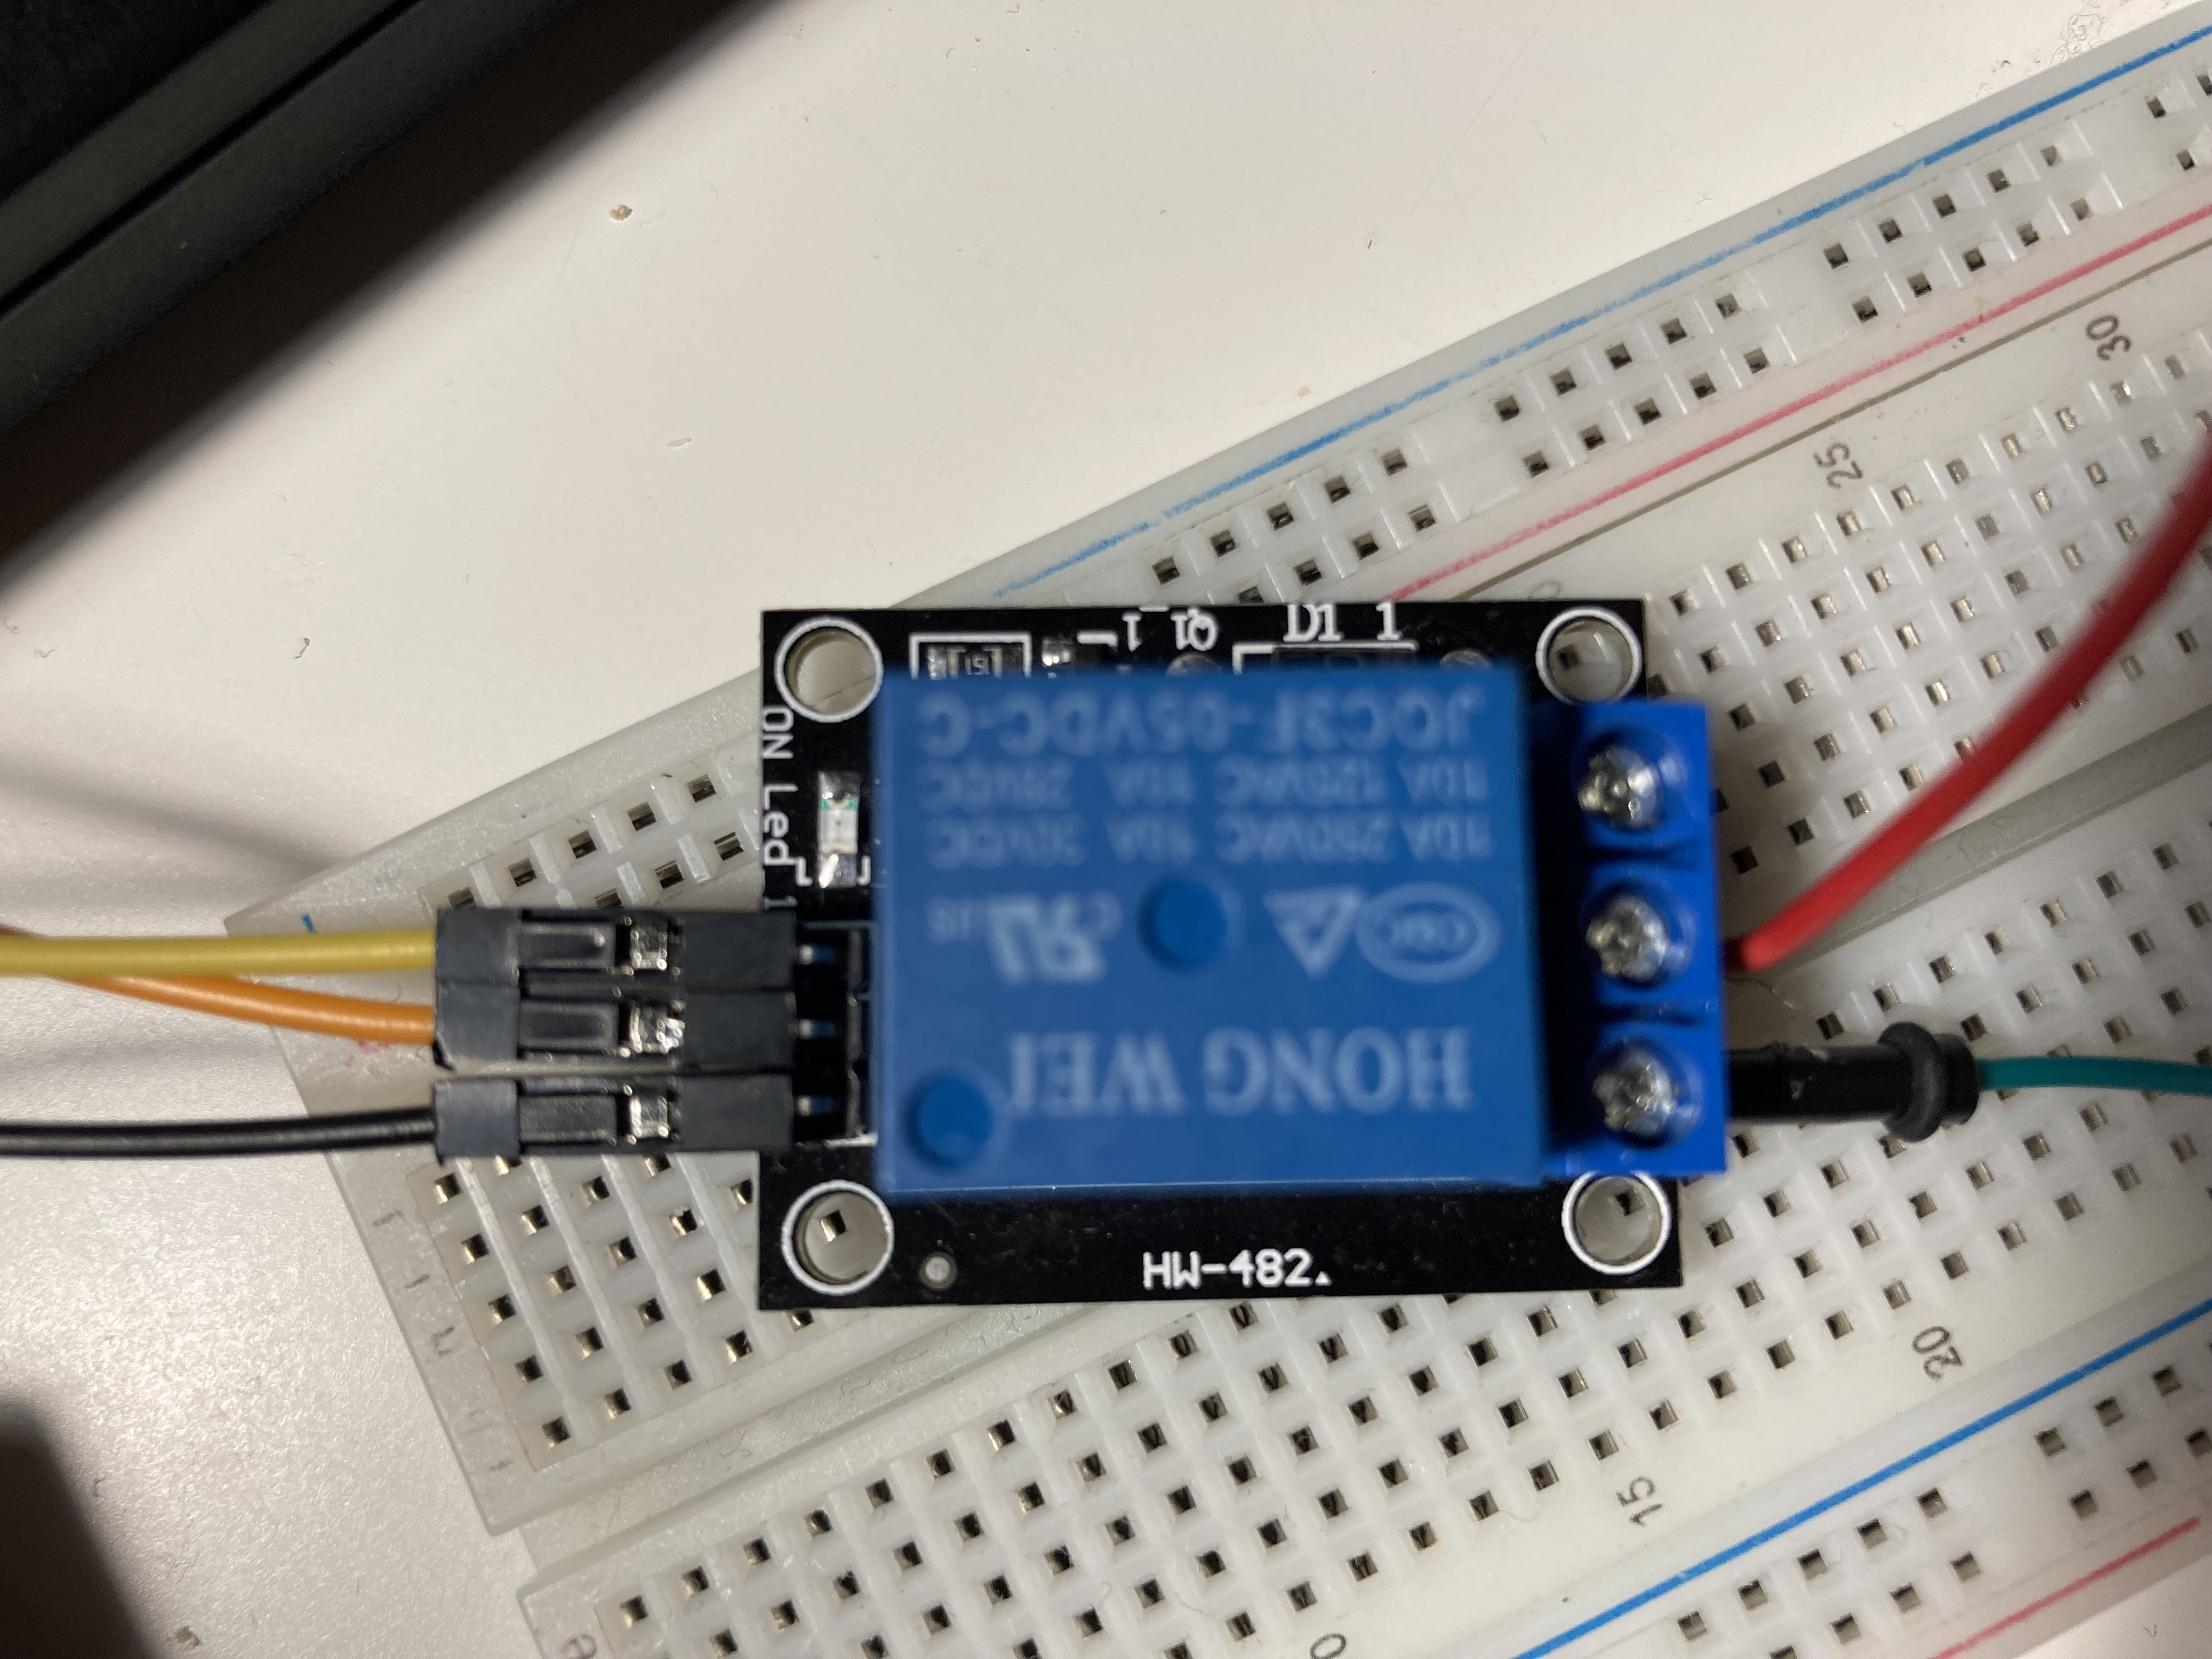
\includegraphics[scale=0.08]{fig/obrazki/działanie_ukladu/bliskof.jpg}
    \caption{nieświecąca się dioda led sygnalizująca brak zasilania pinu s (zółty przewód)}
    \label{fig:my_label}
\end{figure}
\vspace{0.5cm}




\section*{Podsumowanie} \addcontentsline{toc}{section}{Podsumowanie}
Przekaźnik jest urządzeniem o prostym działaniu, takie jest też jego zastosowanie. Sterowanie cewką za pomocą mikrokontrolera NUCLEO-F756ZG wykonujemy za pomocą zmiany stanu jednego z pinów w mikrontrolerze.

\printbibliography[heading=bibintoc]

\end{document}